\documentclass[a4paper,8pt,twocolumn]{article}
\usepackage[UTF8]{ctex}
\usepackage{graphicx}
\usepackage{fancyhdr}
\usepackage{amsmath}
\usepackage{subcaption}
\usepackage{float}
\usepackage[
  left=2cm,
  right=2cm,
  top=1.5cm,
  bottom=2.5cm
]{geometry}
\usepackage{siunitx}
\usepackage{booktabs}
\usepackage{enumitem}
\usepackage{array}
\usepackage{tabularx}
\newcolumntype{Y}{>{\centering\arraybackslash}X}
\usepackage{amssymb}
\usepackage{cancel}
\usepackage{pgfplots}
\usepackage{pgfplotstable}
\pgfplotsset{compat=1.18}

%================ I-V 曲线统一样式 ================
\pgfplotsset{
  ivplot/.style={
    width=0.90\columnwidth,
    height=0.24\textheight,
    scale only axis,
    grid=major,
    enlargelimits=false,
    xlabel={电压 $U$ / \si{V}},
    ylabel={光功率 $W$ / \si{mW}},
    title style={font=\small},
    label style={font=\small},
    ticklabel style={font=\scriptsize},
    legend style={font=\scriptsize, at={(0.98,0.98)},
                  anchor=north east, cells={anchor=west}},
    xmin=0, xmax=1500,
    ymin=0,
  }
}
%===================================================

\sisetup{
  per-mode=symbol,
  separate-uncertainty=true
}

\title{
  \textbf{\huge D1：电光调制及通讯应用}
}
\author{
  黄雨~24352027\\
  \small 中山大学物理学院~广东~广州
}

\pagestyle{fancy}
\fancyhf{}
\fancyhead[C]{D1：电光调制及通讯应用}
\fancyfoot[C]{\thepage}

\begin{document}
\maketitle
\newpage

%%%%%%%%%%%%%%%%%%%%%%%%%%%%%%%%%%%%%%%%%%%%%%%%%%%%%%%%%%%%
\section{实验目的}

\begin{enumerate}
  \item 了解晶体线性电光效应（Pockels效应）的物理原理；
  \item 测量LiNbO$_3$（铌酸锂，LN）晶体横向电光调制的$I$-$V$曲线，实验确定半波电压$V_\pi$；
  \item 插入$\lambda/4$波片后重新测量$I$-$V$曲线，由曲线平移量计算波片光程差并与理论值对比；
  \item 观测并理解"倍频失真"现象，利用失真工作点独立测量$V_\pi$；
  \item 完成模拟光通信实验，理解电光调制在光纤通信中的实际应用。
\end{enumerate}

%%%%%%%%%%%%%%%%%%%%%%%%%%%%%%%%%%%%%%%%%%%%%%%%%%%%%%%%%%%%
\section{实验仪器与装置}

\begin{itemize}
  \item 半导体激光器（$\lambda=\SI{650}{nm}$）；
  \item LiNbO$_3$电光晶体（$L=\SI{30}{mm}$，$d=\SI{5}{mm}$）；
  \item 起偏器与检偏器各一个；
  \item $\lambda/4$波片；
  \item 光功率计（对应波长档位）；
  \item 光电探测器；
  \item 电光控制器（含偏置电压源及正弦波调制信号发生器）；
  \item 双踪示波器（RIGOL）；
  \item 凸透镜（观察锥光干涉图案）；
  \item 小孔光阑、导轨及白屏。
\end{itemize}

%%%%%%%%%%%%%%%%%%%%%%%%%%%%%%%%%%%%%%%%%%%%%%%%%%%%%%%%%%%%
\section{实验原理}

\subsection{线性电光效应与半波电压}

晶体在外加电场下折射率随电场线性变化，称为线性电光效应（Pockels效应）。对于LiNbO$_3$晶体（$3m$对称群），当外电场$E$平行于$x$轴（晶体短边方向）、激光沿$z$轴传播时，由电光张量分量$\gamma_{22}$引起的两本征偏振方向折射率变化分别为
\begin{equation}
  \Delta n_x = +\tfrac{1}{2}n_o^3\gamma_{22}E,\quad
  \Delta n_y = -\tfrac{1}{2}n_o^3\gamma_{22}E
  \tag{D1.1}
\end{equation}
总双折射差$\Delta n = n_o^3\gamma_{22}E$，其中$n_o$为常光折射率，$E=U/d$（$U$为外加电压，$d$为沿电场方向的晶体尺寸）。

光通过长度为$L$的晶体后，两偏振分量的相位差为
\begin{equation}
  \Delta\varphi = \frac{2\pi}{\lambda}\,n_o^3\gamma_{22}\,\frac{U}{d}\cdot L
  \tag{D1.2}
\end{equation}
当$\Delta\varphi=\pi$时，所需电压即\textbf{半波电压}：
\begin{equation}
  V_\pi = \frac{\lambda d}{2n_o^3\gamma_{22}L}
  \tag{D1.3}
\end{equation}

代入参数$\lambda=\SI{650}{nm}$，$n_o=2.297$，$\gamma_{22}=6.8\times10^{-12}$\,m/V，$L=\SI{30}{mm}$，$d=\SI{5}{mm}$：
\begin{align}
  V_\pi &= \frac{\lambda d}{2n_o^3\gamma_{22}L}
  = \frac{3.25\times10^{-9}\,\text{m}^2}{4.945\times10^{-12}\,\text{m/V}}
  \notag\\
  &\approx \SI{657}{V}
  \tag{D1.4}
\end{align}

\subsection{$I$-$V$曲线}

两正交偏振片夹持电光晶体，透射光强为
\begin{equation}
  I(U) = I_0\sin^2\!\!\left(\frac{\pi U}{2V_\pi}+\varphi_0\right)
  \tag{D1.5}
\end{equation}
其中$\varphi_0$为外加电压为零时晶体自然双折射引起的初始相位。曲线呈正弦平方形式，相邻极大（极小）值之间的电压间距为$2V_\pi$，相邻极大与极小之间的间距为$V_\pi$。

\subsection{$\lambda/4$波片的引入}

在晶体与偏振片之间插入$\lambda/4$波片（光轴与偏振方向成$45^\circ$），波片引入额外相位延迟$\Gamma$，使$I$-$V$曲线沿电压轴整体平移$\Delta U$，满足
\begin{equation}
  \Delta U = \frac{\Gamma}{\pi}\,V_\pi
  \tag{D1.6}
\end{equation}
由此可得波片的光程差
\begin{equation}
  \delta = \frac{\Gamma\lambda}{2\pi} = \frac{\Delta U\,\lambda}{2V_\pi}
  \tag{D1.7}
\end{equation}
对理想$\lambda/4$波片，$\Gamma=\pi/2$，$\delta=\lambda/4=\SI{162.5}{nm}$。

\subsection{倍频失真}

设调制信号$u(t)=u_m\sin\omega t$叠加于偏置电压$U_0$，输出光强为
\begin{equation}
  I(t) \propto \sin^2\!\!\left(\frac{\pi(U_0+u_m\sin\omega t)}{2V_\pi}+\varphi_0\right)
  \tag{D1.8}
\end{equation}
当工作点处于$I$-$V$曲线极值（即$\Delta\varphi = k\pi/2$，$k$为奇数时为极大/极小）时，一阶调制项消失，输出信号主要含频率为$2\omega$的成分——此即\textbf{倍频失真}。相邻两个失真点对应电压之差即等于$V_\pi$，可独立用于定标。

%%%%%%%%%%%%%%%%%%%%%%%%%%%%%%%%%%%%%%%%%%%%%%%%%%%%%%%%%%%%
\section{实验步骤}

\subsection{未加$\lambda/4$波片（调光路与测$I$-$V$曲线）}

\begin{enumerate}[label=(\alph*)]
  \item 根据给定参数计算$V_\pi$理论值（见式（D1.4））。
  \item 利用小孔光阑将激光束调节至与导轨平行。
  \item 两偏振片正交放置，插入LN晶体，调节使晶体前后表面反射光与入射光重合（即光轴平行激光束），激光通过晶体中央以消除边缘效应。
  \item 加入凸透镜，检偏器后放白屏，观察\textbf{锥光干涉图案}（图\,\ref{fig:conical}）；调节晶体使激光束斑与黑十字中心重合，旋转两偏振片使黑十字呈水平—竖直方向，确认外加电场方向平行于晶体短边。
  \item 用功率计测量$I$-$V$曲线：从\SI{0}{V}起每隔\SI{10}{V}记录一点，在半波电压附近改为每隔\SI{5}{V}记录一点。
\end{enumerate}

\begin{figure}[H]
  \centering
  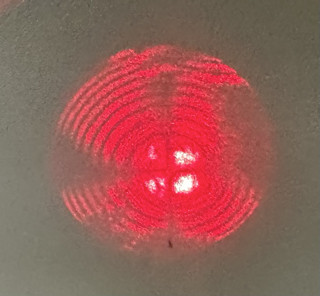
\includegraphics[width=0.55\columnwidth]{锥光干涉图案.png}
  \caption{LN晶体锥光干涉图案：黑十字清晰居中，激光束斑与十字中心重合，表明晶体光轴已与激光束平行。}
  \label{fig:conical}
\end{figure}

\subsection{加入$\lambda/4$波片（通信实验）}

\begin{enumerate}[label=(\alph*),start=6]
  \item 在晶体与偏振片之间插入$\lambda/4$波片，将其光轴调至与偏振片方向成$45^\circ$，重新测量$I$-$V$曲线，记录极值位置变化。（调节方法：旋转波片至$U=0$处透射光强最大时即为$45^\circ$，此时线偏振光被转换为近圆偏振光，$I$-$V$曲线偏移量最大。）
  \item 取下$\lambda/4$波片，换上光电探测器，"信号监测"拨至"内"，用示波器观测不同偏置电压下的输出波形，找出倍频失真最明显处并记录对应偏置电压。
  \item 光路中重新加入$\lambda/4$波片并旋转$360^\circ$，在示波器上观察输入—输出波形随波片方向的变化，以及音频通信实验中出现的"消声—有声"交替现象。
  \item 进行模拟光通信实验：MP3耳机孔接"信号输入"，小音箱接探测器，"信号监测"切换至"外"，调节幅度与偏置电压至音质最清晰（偏置约\SI{595}{V}）。
  \item 实验完毕，旋钮归零，关闭电源，填写设备登记表。
\end{enumerate}

%%%%%%%%%%%%%%%%%%%%%%%%%%%%%%%%%%%%%%%%%%%%%%%%%%%%%%%%%%%%
\section{实验结果与分析}

\subsection{锥光干涉图案}

锥光干涉图案见图\,\ref{fig:conical}。图中黑十字清晰，激光束斑位于十字中心，证明晶体光轴与激光束平行、偏振方向已正确对齐。

\subsection{未加$\lambda/4$波片时的$I$-$V$曲线}

图\,\ref{fig:iv1}为未加$\lambda/4$波片时测得的$I$-$V$曲线。提取极值点如表\,\ref{tab:peaks1}所示。

\begin{table}[H]
\centering
\caption{未加$\lambda/4$波片的$I$-$V$曲线极值}
\label{tab:peaks1}
\begin{tabular}{lcc}
\toprule
极值类型 & $U$ / \si{V} & $W$ / \si{mW} \\
\midrule
第1极大 & 300  & 5.05 \\
第1极小 & 665  & 0.16 \\
第2极大 & 1050 & 5.37 \\
第2极小 & 1420 & 0.24 \\
\bottomrule
\end{tabular}
\end{table}

\noindent\textit{注：$U=\SI{610}{V}$处记录值（$\SI{1.45}{mW}$）与相邻数据严重不符，为测量异常点，绘图时已剔除；$U=370\sim390$\,V区间存在局部波动，可能源于光路微扰。}

\textbf{曲线偏移分析：}理想情形下（两偏振片正交、晶体零场无自然双折射），$U=0$对应透射极小（消光），第一极大应出现在$V_\pi\approx\SI{376}{V}$处。然而实测$I(0)=\SI{0.63}{mW}\neq0$，第一极大出现在$U\approx\SI{300}{V}<V_\pi$，说明晶体存在初始相位偏移$\varphi_0\neq0$。

由式（D1.5），在第一极大处有
\begin{equation}
  \frac{\pi\times300}{2\times376}+\varphi_0 = \frac{\pi}{2}
  \;\Rightarrow\;\varphi_0\approx0.317\,\text{rad}\approx18^\circ
  \tag{D1.9}
\end{equation}
真正的消光点（$I=0$）应在
\begin{equation}
  U_0 = -\varphi_0\cdot\frac{2V_\pi}{\pi}
  \approx -\frac{0.317\times752}{\pi}\approx-\SI{76}{V}
  \tag{D1.10}
\end{equation}
即测量范围之外的负电压处。相应地，零场透射光强的预测值为
$I_0\sin^2\varphi_0\approx5.37\times0.097\approx\SI{0.52}{mW}$，与实测$\SI{0.63}{mW}$相符。

此初始相位$\varphi_0$的来源主要有：
\begin{enumerate}[noitemsep,topsep=2pt]
  \item 晶体$c$轴与激光束方向存在微小偏斜，传播方向上出现残余双折射分量；
  \item 晶体装夹引起的机械应力双折射（光弹效应）；
  \item 偏振片与晶体$x$/$y$轴的调节未达到理想正交。
\end{enumerate}

由相邻极值位置提取$V_\pi$：
\begin{align}
  V_\pi^{(1)} &= \frac{(1050-300)+(1420-665)}{4}
  \notag\\
  &= \frac{750+755}{4} \approx \SI{376}{V}
  \tag{D1.11}
\end{align}

\begin{figure}[H]
  \centering
  \begin{tikzpicture}
  \begin{axis}[
    ivplot,
    ymax=6.5,
    title={未加$\lambda/4$波片的$I$-$V$曲线},
  ]
    \addplot[mark=none,blue,thick,line width=0.8pt] coordinates {
      (0,0.63)(10,0.76)(20,0.95)(30,1.12)(40,1.25)(50,1.36)
      (60,1.53)(70,1.73)(80,1.82)(90,1.95)(100,2.09)(110,2.30)
      (120,2.75)(130,3.05)(140,3.05)(150,3.17)(160,3.28)(170,3.47)
      (180,3.73)(190,3.91)(200,4.12)(210,4.21)(220,4.30)(230,4.47)
      (240,4.63)(250,4.76)(260,4.84)(270,4.91)(280,4.95)(290,5.02)
      (300,5.05)(310,5.02)(320,4.98)(330,4.92)(340,4.81)(350,4.55)
      (360,4.23)(370,4.03)(380,4.33)(390,4.38)(400,4.28)(410,4.07)
      (420,3.77)(430,3.53)(440,3.25)(450,2.98)(460,2.75)(470,2.53)
      (480,2.32)(490,2.13)(500,1.89)(510,1.70)(520,1.55)(530,1.45)
      (540,1.41)(550,1.32)(560,1.27)(570,1.15)(580,1.04)(590,0.80)
      (600,0.62)(620,0.38)(630,0.23)(640,0.19)(650,0.17)
      (660,0.16)(670,0.16)(680,0.18)(690,0.23)(700,0.29)
      (710,0.33)(720,0.41)(730,0.50)(740,0.59)(750,0.70)
      (760,0.84)(770,0.99)(780,1.14)(790,1.35)(800,1.54)
      (810,1.72)(820,1.85)(830,2.05)(840,2.19)(850,2.34)
      (860,2.52)(870,2.85)(880,3.26)(890,3.50)(900,3.71)
      (910,3.72)(920,3.85)(930,4.04)(940,4.22)(950,4.40)
      (960,4.59)(970,4.76)(980,4.83)(990,4.92)(1000,5.01)
      (1010,5.08)(1020,5.13)(1030,5.19)(1040,5.28)(1050,5.37)
      (1060,5.31)(1070,5.20)(1080,5.09)(1090,5.01)(1100,4.92)
      (1110,4.81)(1120,4.77)(1130,4.66)(1140,4.58)(1150,4.53)
      (1160,4.38)(1170,4.28)(1180,4.01)(1190,3.80)(1200,3.65)
      (1210,3.45)(1220,3.25)(1230,2.99)(1240,2.72)(1250,2.46)
      (1260,2.20)(1270,1.92)(1280,1.70)(1290,1.49)(1300,1.25)
      (1310,1.07)(1320,0.92)(1330,0.79)(1340,0.67)(1350,0.57)
      (1360,0.46)(1370,0.39)(1380,0.32)(1390,0.29)(1400,0.27)
      (1410,0.25)(1420,0.24)(1430,0.25)(1440,0.29)(1450,0.36)
      (1460,0.45)(1470,0.55)(1480,0.68)(1490,0.79)
    };
    \addplot[only marks,mark=triangle*,mark size=2.5pt,red] coordinates {
      (300,5.05)(665,0.16)(1050,5.37)(1420,0.24)
    };
    \legend{实测数据, 极值点}
  \end{axis}
  \end{tikzpicture}
  \caption{未加$\lambda/4$波片的$I$-$V$曲线（蓝线），红三角为极值点。曲线偏移使真正消光点在$U\approx-\SI{76}{V}$处（测量范围外）。$U=\SI{610}{V}$处异常点已剔除。}
  \label{fig:iv1}
\end{figure}

\subsection{加入$\lambda/4$波片后的$I$-$V$曲线及光程差}

\textbf{波片45°放置方法：}将$\lambda/4$波片插入起偏器与晶体之间，初始令波片主轴与起偏器偏振方向平行（$0^\circ$），此时波片不改变线偏振态，$I$-$V$曲线与未加波片时相同。缓慢旋转波片并监测$U=0$处的透射光强：当主轴与偏振方向平行或垂直（$0^\circ$或$90^\circ$）时，输出接近消光；当旋转至$45^\circ$时，线偏振光被转换为（近似）圆偏振光，$I(0)$达到最大，$I$-$V$曲线整体平移量最大。以$I(0)$最大处作为$45^\circ$的判据，并进一步核查$I$-$V$曲线极小值移动量是否接近$V_\pi/2$（理想$\lambda/4$波片对应）以验证正确性。

图\,\ref{fig:iv2}为加入$\lambda/4$波片后测得的$I$-$V$曲线，曲线整体向低电压方向平移，起始光强$I(0)\approx\SI{3.10}{mW}$接近极大值，说明零电压处工作点已从消光位置移至近极大位置，与插入$\lambda/4$波片的预期一致。极大值降至$\approx\SI{3.47}{mW}$（较未加波片时小，部分源于波片插入损耗及激光功率的会话间差异）。提取极值点见表\,\ref{tab:peaks2}。

\begin{table}[H]
\centering
\caption{加入$\lambda/4$波片后的$I$-$V$曲线极值}
\label{tab:peaks2}
\begin{tabular}{lcc}
\toprule
极值类型 & $U$ / \si{V} & $W$ / \si{mW} \\
\midrule
第1极大 & 20  & 3.25 \\
第1极小 & 415 & 0.14 \\
第2极大 & 800 & 3.47 \\
第2极小 & 1180 & 0.14 \\
\bottomrule
\end{tabular}
\end{table}

由相邻极值间距再次估算半波电压：
\begin{align}
  V_\pi^{(2)} &= \frac{(800-20)+(1180-415)}{4}
  \notag\\
  &= \frac{780+765}{4} \approx \SI{386}{V}
  \tag{D1.12}
\end{align}

\begin{figure}[H]
  \centering
  \begin{tikzpicture}
  \begin{axis}[
    ivplot,
    ymax=4.5,
    title={加入$\lambda/4$波片后的$I$-$V$曲线},
  ]
    \addplot[mark=none,red!70!black,thick,line width=0.8pt] coordinates {
      (0,3.10)(10,3.21)(20,3.25)(30,3.19)(40,3.12)(50,3.08)
      (60,2.98)(70,2.94)(80,2.90)(90,2.85)(100,2.81)(110,2.76)
      (120,2.68)(130,2.56)(140,2.45)(150,2.33)(160,2.21)(170,2.06)
      (180,1.90)(190,1.78)(200,1.67)(210,1.57)(220,1.48)(230,1.39)
      (240,1.32)(250,1.21)(260,1.08)(270,1.02)(280,0.95)(290,0.89)
      (300,0.84)(310,0.76)(320,0.68)(330,0.58)(340,0.48)(350,0.39)
      (360,0.32)(370,0.25)(380,0.20)(390,0.17)(400,0.15)(410,0.14)
      (420,0.14)(430,0.16)(440,0.19)(450,0.23)(460,0.28)(470,0.34)
      (480,0.40)(490,0.47)(500,0.55)(510,0.65)(520,0.76)(530,0.87)
      (540,0.99)(550,1.09)(560,1.22)(570,1.39)(580,1.50)(590,1.60)
      (600,1.71)(610,1.82)(620,1.92)(630,2.01)(640,2.10)(650,2.21)
      (660,2.32)(670,2.42)(680,2.50)(690,2.55)(700,2.57)(710,2.67)
      (720,2.79)(730,2.86)(740,2.94)(750,3.01)(760,3.13)(770,3.25)
      (780,3.40)(790,3.46)(800,3.47)(810,3.45)(820,3.37)(830,3.30)
      (840,3.21)(850,3.10)(860,3.03)(870,2.96)(880,2.85)(890,2.78)
      (900,2.73)(910,2.66)(920,2.57)(930,2.47)(940,2.37)(950,2.25)
      (960,2.14)(970,2.02)(980,1.87)(990,1.76)(1000,1.67)(1010,1.61)
      (1020,1.48)(1030,1.31)(1040,1.20)(1050,1.08)(1060,0.95)(1070,0.80)
      (1080,0.60)(1090,0.51)(1100,0.42)(1110,0.36)(1120,0.31)(1130,0.27)
      (1140,0.23)(1150,0.20)(1160,0.17)(1170,0.15)(1180,0.14)(1190,0.15)
      (1200,0.16)(1210,0.18)(1220,0.21)(1230,0.25)(1240,0.31)(1250,0.37)
      (1260,0.47)(1270,0.57)(1280,0.71)(1290,0.88)(1300,1.01)(1310,1.13)
      (1320,1.23)(1330,1.31)(1340,1.38)(1350,1.47)(1360,1.57)(1370,1.68)
      (1380,1.81)(1390,1.92)(1400,2.01)(1410,2.12)(1420,2.34)(1430,2.60)
      (1440,2.77)(1450,2.86)(1460,2.84)(1470,2.72)(1480,2.83)(1490,2.93)
    };
    \addplot[only marks,mark=triangle*,mark size=2.5pt,blue!80!black] coordinates {
      (20,3.25)(415,0.14)(800,3.47)(1180,0.14)
    };
    \legend{实测数据, 极值点}
  \end{axis}
  \end{tikzpicture}
  \caption{加入$\lambda/4$波片后的$I$-$V$曲线（红线），蓝三角为极值点。曲线整体向低压平移，起点$I(0)\approx\SI{3.10}{mW}$接近极大值。}
  \label{fig:iv2}
\end{figure}

\textbf{波片光程差：}对比两周对应极值点位置，极大值从$\SI{300}{V}$移至$\SI{20}{V}$（$\Delta U_{\max}=\SI{280}{V}$），极小值从$\SI{665}{V}$移至$\SI{415}{V}$（$\Delta U_{\min}=\SI{250}{V}$），取均值$\overline{\Delta U}=\SI{265}{V}$（与实验记录所估$\SI{300}{V}$相近）。由式（D1.7）得波片光程差：
\begin{equation}
  \delta = \frac{\overline{\Delta U}\cdot\lambda}{2V_\pi^{(1)}}
  = \frac{265\times\SI{650}{nm}}{2\times376}
  \approx \SI{229}{nm}
  \tag{D1.13}
\end{equation}
该值约为理论值$\lambda/4=\SI{162.5}{nm}$的$1.41$倍，即此波片对\SI{650}{nm}激光的实际延迟量约为$0.35\lambda$，表明该波片并非严格意义上的$\lambda/4$波片，可能因设计波长与本实验激光波长不同所致。

\subsection{倍频失真观测}

图\,\ref{fig:dist307}与图\,\ref{fig:dist701}为（未加$\lambda/4$波片时）偏置电压分别为$\SI{307}{V}$和$\SI{701}{V}$时示波器拍摄的波形。黄色通道（CH1，$\SI{5}{V/div}$）为正弦波调制输入信号，青色通道（CH2）为探测器输出信号。

两图中，CH2输出频率均约为CH1的两倍。偏置$\SI{307}{V}$对应未加$\lambda/4$波片时$I$-$V$曲线的极大值（约$\SI{300}{V}$），工作点处于透射率饱和区；偏置$\SI{701}{V}$对应极小值（约$\SI{665}{V}$），工作点处于透射率零区；两者均使一阶调制消失，出现倍频。

\textbf{峰形特征：}当偏置电压\emph{精确}位于极值时，$I$-$V$曲线对工作点左右对称，输出$2\omega$信号正负半周幅度相等，CH2波形呈\emph{等高双峰}（纯倍频）——这是失真最明显的特征。若将偏置稍作调节使工作点偏离极值，则一阶分量重新出现，CH2波形中两相邻峰高低不一（一峰高、一峰低交替），调制失真介于线性调制与纯倍频之间。利用此特征可精确定位极值位置：调节偏置至CH2恰好出现等高双峰时的电压即对应极值，两相邻极值之差即为$V_\pi$。

\begin{figure}[H]
  \centering
  \includegraphics[width=0.95\columnwidth]{倍频失真_307V.png}
  \caption{$U_0=\SI{307}{V}$时的倍频失真（极大值工作点）：CH1为输入正弦波，CH2为频率翻倍的输出信号（$\SI{50}{V/div}$）。}
  \label{fig:dist307}
\end{figure}

\begin{figure}[H]
  \centering
  \includegraphics[width=0.95\columnwidth]{倍频失真_701V.png}
  \caption{$U_0=\SI{701}{V}$时的倍频失真（极小值工作点）：CH1为输入正弦波，CH2为频率翻倍的输出信号（$\SI{20}{V/div}$）。}
  \label{fig:dist701}
\end{figure}

由相邻失真点计算$V_\pi$：
\begin{equation}
  V_\pi^{(\text{dist})} = U_{0,\min} - U_{0,\max} = 701 - 307 = \SI{394}{V}
  \tag{D1.14}
\end{equation}

\subsection{模拟光通信：旋转$\lambda/4$波片的有声—消声分布}

加入$\lambda/4$波片并施加约$\SI{595}{V}$偏置后，以音频信号作为调制输入，旋转波片一周（$0^\circ$--$360^\circ$）记录音频清晰（有声）与严重失真（消声）的角度，如图\,\ref{fig:rotation}所示。

\begin{figure}[H]
  \centering
  \begin{tikzpicture}[scale=0.88]
    % Main circle
    \draw[thick] (0,0) circle(2.0cm);
    % Dashed axis lines
    \draw[gray,dashed] (-2.55,0)--(2.55,0);
    \draw[gray,dashed] (0,-2.55)--(0,2.55);
    % Tick marks every 30°
    \foreach \a in {0,30,...,330} {
      \draw[gray!70] (\a:1.93cm)--(\a:2.07cm);
    }
    % Cardinal labels
    \node[font=\scriptsize] at (2.68,0) {$0^\circ$};
    \node[font=\scriptsize] at (0,2.42) {$90^\circ$};
    \node[font=\scriptsize] at (-2.75,0) {$180^\circ$};
    \node[font=\scriptsize] at (0,-2.42) {$270^\circ$};
    % Sound angles (有聲): blue filled circles, labels at 2.45cm
    \foreach \ang in {30,60,90,150,200,240,270} {
      \fill[blue!80!black] (\ang:2.0cm) circle(2.8pt);
      \node[font=\tiny,blue!80!black] at (\ang:2.46cm) {\ang};
    }
    % Silent angles (消聲): red ×, labels at 2.80cm
    \foreach \ang in {40,70,120,170,230,250,290} {
      \node[red,font=\small,inner sep=0pt] at (\ang:2.0cm) {$\times$};
      \node[font=\tiny,red] at (\ang:2.80cm) {\ang};
    }
    % Legend
    \fill[blue!80!black] (-0.95,-2.68) circle(2.8pt);
    \node[right,font=\scriptsize] at (-0.80,-2.68) {有声};
    \node[red,font=\small,inner sep=0pt] at (-0.95,-3.08) {$\times$};
    \node[right,font=\scriptsize] at (-0.80,-3.08) {消声};
  \end{tikzpicture}
  \caption{旋转$\lambda/4$波片一周时的有声—消声分布（偏置$\approx\SI{595}{V}$）。蓝色实心圆为音频清晰的有声角度（$30^\circ,60^\circ,90^\circ,150^\circ,200^\circ,240^\circ,270^\circ$），红色"$\times$"为严重失真的消声角度（$40^\circ,70^\circ,120^\circ,170^\circ,230^\circ,250^\circ,290^\circ$）。}
  \label{fig:rotation}
\end{figure}

有声与消声位置交替出现，且各对有声—消声之间仅相差约$10^\circ\sim30^\circ$，说明从"线性工作点"到"极值工作点"之间的过渡极为敏感。每约$90^\circ$出现一对有声—消声，与$\lambda/4$波片旋转时等效相位偏移$\Gamma_\text{eff}=(\pi/2)\sin2\theta$每$90^\circ$完成一个半周期的规律一致。偏置$\SI{595}{V}$大致对应有聲光路中的二次极大与极小之间的正交（线性）工作点，波片旋转使有效初相在正交点与极值之间往返，从而产生周期性的清晰—失真切换。

\subsection{综合比较与误差分析}

\begin{table}[H]
\centering
\caption{各方法所得$V_\pi$汇总}
\label{tab:summary}
\begin{tabularx}{\columnwidth}{lY}
\toprule
方法 & $V_\pi$ / \si{V} \\
\midrule
理论计算（式D1.3） & 657 \\
未加$\lambda/4$波片极值法 & 376 \\
加入$\lambda/4$波片极值法 & 386 \\
倍频失真点法 & 394 \\
实验均值 & 385 \\
\bottomrule
\end{tabularx}
\end{table}

三种实验方法所得$V_\pi$互差小于$\SI{5}{\percent}$，一致性良好，说明测量重复性高、随机误差小。然而实验均值$\SI{385}{V}$与理论值$\SI{657}{V}$相差约$\SI{41}{\percent}$，偏低显著，可能原因如下：

\begin{enumerate}
  \item \textbf{材料参数差异：}实际LN晶体的$n_o$和$\gamma_{22}$因掺杂、温度、制备工艺与常用文献值存在偏差；实验记录中$n_o=2.247$（文献常见为$2.28$--$2.30$），亦反映出参数不确定性。
  \item \textbf{电场非均匀性：}横向调制中电场在$d$方向并不完全均匀，边缘效应使有效作用场大于$U/d$，导致实际$V_\pi$偏小。
  \item \textbf{取向误差：}若晶体$x$轴与外加电场方向存在小角偏差，等效电光系数将偏离$\gamma_{22}$；实验中的对准精度有限。
  \item \textbf{公式理想化：}式（D1.3）基于完全横向、均匀场及无自然双折射偏移的理想模型，实际情形与之有偏差。
\end{enumerate}

%%%%%%%%%%%%%%%%%%%%%%%%%%%%%%%%%%%%%%%%%%%%%%%%%%%%%%%%%%%%
\section{思考题}

\begin{enumerate}

\item \textbf{计算纵向调制（以KDP为例）的半波电压表达式，并证明其与晶体尺寸无关。}

对于KDP（KH$_2$PO$_4$，$\bar{4}2m$对称群）纵向调制，电场$E_z$沿光传播方向（$z$轴）施加。由电光系数$r_{63}$引起的折射率椭球变化，在$x'y'$截面产生感生双折射：
\begin{equation}
  \Delta n_{x'} = +\tfrac{1}{2}n_o^3r_{63}E_z,\quad
  \Delta n_{y'} = -\tfrac{1}{2}n_o^3r_{63}E_z
  \tag{D1.15}
\end{equation}
两本征偏振分量经长度$L$晶体后的相位差为
\begin{equation}
  \Delta\varphi = \frac{2\pi}{\lambda}\,n_o^3 r_{63}\,E_z\cdot L
  = \frac{2\pi}{\lambda}\,n_o^3 r_{63}\,\frac{U}{\cancel{L}}\cdot \cancel{L}
  = \frac{2\pi n_o^3 r_{63}}{\lambda}\,U
  \tag{D1.16}
\end{equation}
关键之处在于：纵向调制中$E_z = U/L$，代入后晶体长度$L$完全相消。令$\Delta\varphi=\pi$，得
\begin{equation}
  \boxed{V_\pi^{(\mathrm{KDP})} = \frac{\lambda}{2n_o^3 r_{63}}}
  \tag{D1.17}
\end{equation}
结果\textbf{仅依赖于光波长和材料常数，与晶体长度$L$及截面尺寸$d$均无关}。物理根源：晶体加长使相互作用路径增大，但相同电压在更长晶体中产生更弱的场（$E=U/L$），两效应恰好相消。

以KDP常用参数（$\lambda=\SI{650}{nm}$，$n_o\approx1.51$，$r_{63}\approx\SI{10.6}{pm/V}$）估算：
\begin{equation}
  V_\pi^{(\mathrm{KDP})} \approx \frac{650\times10^{-9}}{2\times(1.51)^3\times10.6\times10^{-12}}
  \approx \SI{8.4}{kV}
  \notag
\end{equation}
可见纵向调制的$V_\pi$高达数kV，远大于横向调制（数百V），这正是其主要缺点——需要很高的驱动电压。

\item \textbf{如果晶体光轴与激光束不平行，或$x$/$y$轴与偏振片不平行，如何检查？对测量结果有何影响？}

\textbf{检查方法：}

（1）\textit{光轴与激光束偏斜：}在检偏器后加白屏并置凸透镜，观察锥光干涉图案。正确对准时黑十字中心与激光束斑严格重合；若光轴偏斜，十字中心偏移束斑，且干涉环不再圆对称。可微调晶体俯仰与横向位置，使束斑归回十字中心。

（2）\textit{$x$/$y$轴与偏振片方向偏斜：}锥光干涉图案的黑十字两臂应分别平行于起偏器和检偏器的偏振方向（即水平—竖直）。若晶体$x$轴旋转了角度$\theta$，十字整体偏转$\theta$。通过共同旋转两偏振片（保持相互正交）直至十字恢复水平—竖直，即可修正。

\textbf{对测量结果的影响：}

（1）\textit{光轴偏斜：}光在晶体内产生走离效应（walk-off），有效相互作用长度缩短；同时自然双折射的贡献增大，导致$\varphi_0$偏大，$I$-$V$曲线起点偏离零值，消光比下降，极值位置出现额外偏移，使测得$V_\pi$产生系统误差。

（2）\textit{$x$/$y$轴与偏振方向偏斜$\theta$角：}起作用的电光系数变为$\gamma_{22}\cos2\theta$，有效系数减小，导致测得$V_\pi$偏大（晶体表观调制能力下降）。同时，$I$-$V$曲线的调制深度（极大与极小之比，即消光比）降低，使极值读数模糊，进一步增大$V_\pi$的测量不确定度。

\end{enumerate}

%%%%%%%%%%%%%%%%%%%%%%%%%%%%%%%%%%%%%%%%%%%%%%%%%%%%%%%%%%%%
\clearpage
\onecolumn
\section*{参考文献}

\begin{enumerate}[label={[\arabic*]}]
  \item 赵凯华，钟锡华. 光学（下册）[M]. 北京：北京大学出版社，1984：326--340.
  \item Yariv A, Yeh P. Photonics: Optical Electronics in Modern Communications [M]. 6th ed. Oxford: Oxford University Press, 2007: 250--280.
  \item Saleh B E A, Teich M C. Fundamentals of Photonics [M]. 3rd ed. New York: Wiley, 2019: 771--795.
  \item 中山大学物理实验教学中心. D1电光调制实验说明书 [Z]. 广州：中山大学，2024.
\end{enumerate}

\clearpage

\section{教师签名页}
\begin{figure}[htbp]
  \centering
  
\includegraphics[width=0.65\textwidth]{签名页.png}
  \caption{教师签名页}
\end{figure}

\end{document}
